\Chapter{Introduction}
%%%%%%%%%%%%%%%%%%%%%%%%%%%%%%%%%%%%%%%%%%%%%%%%%%%%%%%%%%%%%%%%%%%%%%%%%%%%%%%%%%%%%%%%%%%%
%%%%%%%%%%%%%%%%%%%%%%%%%%%%%%%%%%%%%%%%%%%%%%%%%%%%%%%%%%%%%%%%%%%%%%%%%%%%%%%%%%%%%%%%%%%%
\Section{Motivation} \label{sec:motivation}
%%%%%%%%%%%%%%%%%%%%%%%%%%%%%%%%%%%%%%%%%%%%%%%%%%%%%%%%%%%%%%%%%%%%%%%%%%%%%%%%%%%%%%%%%%%%
%%%%%%%%%%%%%%%%%%%%%%%%%%%%%%%%%%%%%%%%%%%%%%%%%%%%%%%%%%%%%%%%%%%%%%%%%%%%%%%%%%%%%%%%%%%%
\lsnote{The introduction needs more perspective on what consitutes `high gradient'.  It would be good if you mentioned the typical gradients/limitations of conventional accelerating structures, and mention that they are powered by Klystrons etc.  In other words, you need the broader context in the introduction.}

A new generation of accelerators dedicated to High Energy Physics
(HEP), would likely be of the TeV scale. Reduction in the size and cost
of such machines is key to their feasibility. \lsnote{One scheme that may potentially achieve this is \sout{and can be accomplished
through accelerator technology R\&D. Investigation into a 
high gradient candidate for future HEP machines is an active research area
 A } a}
short pulse, two-beam acceleration (TBA) scheme using 
wakefield power extractors\lsnote{such as that being developed } at the Argonne Wakefield Accelerator (AWA) facility. \lsnote{\sout{Investigation into a 
high gradient candidate for future HEP machines is an active research area
at the Argonne Wakefield Accelerator (AWA) facility. and accelerating structures made 
of metallic materials was demonstrated~\cite{recent-tba}.}}
A goal of the AWA group is to demonstrate fully staged TBA, 
achieving a gradient of 250 MV/m. If successful, this would
be the only facility in the world capable of such gradients used for
acceleration of a beam.

TBA requires a drive beam to pass through a decelerating structure and
\lsnote{lose \sout{loss of}} energy through wakefield generation. The electromagnetic wake
is coupled from the decelerator into an accelerating structure, where
the electric field is used to accelerate a second beam. 
This requires two complete and separate beamlines 
operating synchronously with each other.  
The wakefield structures can be metallic or dielectric on either beam line. 
Dielectric structures, having no irises, are simple to manufacture and have demonstrated
high gradient capability at \SI{100}{MV/m} \cite{WeiPaper}. 

The Compact Linear Collider (CLIC) collaboration, proposes a similar TBA scheme with
a \SI{240}{ns} pulse design. This limits the acceleration gradient
to roughly \SI{150}{MV/m} at room temperature due to rf breakdown \cite{CLICdesignReport}.
Higher gradients could be reached when driven by a very short drive
beam pulse, such as the 20ns pulse length proposed by AWA \cite{WeiPaper}. 
While the peak power and gradients are considerably larger in the short pulse scheme, 
the average power is still feasible and within current technology capabilities.
While the two groups vary on approach, they agree that TBA would 
require less infrastructure when constructing a linear TeV scale machine, 
versus the cost of more conventional technology. 

For example, a case study was done comparing the infrastructure 
needed when using traditional \SI{50}{MW} klystron sources.
It would take roughly 35,000 klystrons to construct a linear machine to deliver the same 
\SI{9.2}{TW} power required in the CLIC design specification reports \cite{CLICdesignReport}. 
With TBA, CLIC projected a \SI{3}{TeV} energy at a length of \SI{48}{km}.
%In contrast to CLIC's 48 km projected machine length needed to reach \SI{3}{TeV}, 
In contrast, the Next Linear Collider (NLC) collaboration projected a \SI{1}{TeV} machine 
with length \SI{26}{km}, using X-band klystrons \cite{NLC}. 
This drastic difference occurs in the infrastructure needed to generate and transfer
RF power in the two cases. In TBA, a high charge bunch train is generated in 
a photoinjector and propagated down stream using conventional technology 
(accelerating structures, quads, dipoles, etc). After it has reached the design energy
is focused into specially designed wakefield structures (decelerating structure).
The RF is then generated in the decelerating structure and supplied to the witness 
beam line through a waveguide connection. This has two benefits over traditional klystron technology.
One, you can have structures at higher frequencies (any multiple of the machine frequency), 
which helps push the gradient. Readily available and production klystrons are limited in this aspect.
Second, all the waveguide infrastructure needed to connect a klystron to the accelerating 
structures is eliminated. There is the initial cost near the photoinjector, 
but downstream, much of the infrastructure costs are eliminated.
Theoretically, TBA can deliver the same amount of power as conventional methods with less 
infrastructure, and therefore lower cost, in the case of a large machine. 

Before a detailed understanding of the power and infrastructure trade offs 
can be obtained, the feasibility of staged TBA must be be demonstrated.
Demonstration of staging is especially important, 
as no high energy machine can be built without staging.
Staging is the ability to use two successive accelerating modules to synchronously accelerate 
the same particle bunch. While simple in principle, the difficulties 
in achieving staging should not be underestimated. 
Demonstration of staging proves that a TBA scheme can be scaled to high energies, and whether it is 
feasible to use such methods. Single stage TBA, and staging 
in a simplified scheme have been demonstrated at the AWA in 2016 \cite{tba2017}.
In the simplified scheme, both bunch trains travel through two decelerating stages.
This causes energy loss in stage 1 as the the second bunch train travels to stage 2.
\nrnote{add figure here to show difference between simplified and full staging}

Fully staged TBA introduces a fast rise time kicker
and subsequent dogleg-like beam line. In this scenario, bunch trains can be 
be directed to two independent decelerating structures. 
Therefore you can extract the maximum amount of power in each stage.
Experimental preparations, design, optimization, 
and initial testing of the fully staged beam line
is the subject of this thesis. 

\lsnote{First, summarize here what main work you did for the thesis.  Then, you can describe what is to come in the thesis to follow: e.g. `Chapter 2 presents'.  This would be the end of the introductory chapter.\\
Non-independent staging power measurments\\
Kicker specification and testing\\
Kicker beamline simulation and optimization : \\
optimization studies, optics settings, phase settings, experimental measurements}

Experimental work included UV laser pulse train improvement, 
which improves the RF power generation in the wakefield structures.
\nrnote{I will add more details to this summary paragraph}
An image processing script was written in Python to analyze YAG screen data. 
A vast number of simulations were performed in OPAL-t~\cite{opal}.
The photoinjector was optimized for \SI{40}{nC}, 
which improved the beam parameters entering the TBA experimental area.
Simulations of the TBA beam line were done to ensure transmission at
the wakefield structure. Optimization of the optics was done using 
a genetic algorithm. 
Experimental results and comparison to simulations, along 
with the following beam dynamics analysis is shown here.

%%%%%%%%%%%%%%%%%%%%%%%%%%%%%%%%%%%%%%%%%%%%%%%%%%%%%%%%%%%%%%%%%%%%%%%%%%%%%%%%
%%%%%%%%%%%%%%%%%%%%%%%%%%%%%%%%%%%%%%%%%%%%%%%%%%%%%%%%%%%%%%%%%%%%%%%%%%%%%%%%
\Section{Argonne Wakefield Accelerator Facility} \label{sec:facility}
%%%%%%%%%%%%%%%%%%%%%%%%%%%%%%%%%%%%%%%%%%%%%%%%%%%%%%%%%%%%%%%%%%%%%%%%%%%%%%%%
%%%%%%%%%%%%%%%%%%%%%%%%%%%%%%%%%%%%%%%%%%%%%%%%%%%%%%%%%%%%%%%%%%%%%%%%%%%%%%%%

\iffalse
\nrnote{this paragraph is from NAPAC paper}
The AWA facility houses a 70 MeV RF photoinjector \cite{upgrades} with a large 
dynamic range: 20 pC to 100 nC. In many cases, the beam is SC dominated. 
In the AWA’s Emittance Exchange (EEX) beam line \cite{eex}, CSR has a large  
effect on the beam as it passes through the dipoles, and wakefields
are present in the two beam acceleration (TBA) beam line \cite{staging1}. ASTRA, 
GPT, and OPAL-T are capable of simulating 3D SC, and wakefield effects.
The latter two codes also include a CSR model, making them a good fit for the AWA.  
\fi

The AWA facility houses two rf photoinjector electron guns operating
at \SI{1.3}{GHz}, and three subsequent beam lines. 
Two of the beam lines are currently used for staged TBA, and the
third is used for Emittance Exchange experiments (EEX). A layout of
the facility is shown in Fig. \ref{fig:bunker}. 
\lsnote{Some more detail will be needed here, maybe just switch the order of the some of the text in the two paragraphs below.  Something like; start with saying what the beamlines are and what is in them referring to the figure, then describe their sources in more detail (RF guns and photocathodes), then talk about the laser and how it is split.}

Electron bunches in a photoinjector are created through the photoelectric effect. 
At the AWA, a pulsed UV laser is propagated through two relay lines of UV optics to either
the drive or witness gun. An in-vacuum mirror then directs the pulse to the photocathode.
Both beam lines must be operated simultaneously when the TBA experiments are run. This is accomplished by
splitting the original laser pulse into two pulses using a UV splitter on the 
ceiling of the bunker. One of the split pulses is sent (as is) to the witness beam line for one
bunch operation. The second pulse is sent to a UV multispitter table, shown in 
Fig.~\ref{fig:optics} where it is split into trains of various lengths. Eight pulses are 
used for TBA drive trains, 

The beam line located on the right side of Fig. \ref{fig:bunker} is called the
drive line. The rf photoinjector on the drive line uses a semiconducting
CsTe cathode, and is followed by a linear accelerator (linac). The
drive linac uses six copper cavities and four klystrons to accelerate the drive beam
to energies of 50-\SI{70}{MeV}. The number of bunches generated from each 
laser pulse can vary from 1, 2, 4, 6, and 8 bunches. When multiple bunches
are generated, the grouping is called a bunch train. Generation of
these variable bunch trains is accomplished by splitting the pulsed
UV laser beam before it enters the gun and hits the cathode. The splitting
takes place in a complex network of UV optics located near the drive
gun. The optics set up is called a beam splitter, or mulitsplitter,
and trains are created at a rate of 0.5, 1, or \SI{2}{Hz}. This timing is
called a pulse, or the repetition rate of the machine. A picture of
the AWA multisplitter table is shown in Fig. \ref{fig:optics}. Optimization 
of the UV optics was performed and is detailed in Section \ref{sec:uvoptics}.  

\iffalse
\begin{figure}
	\begin{center}
		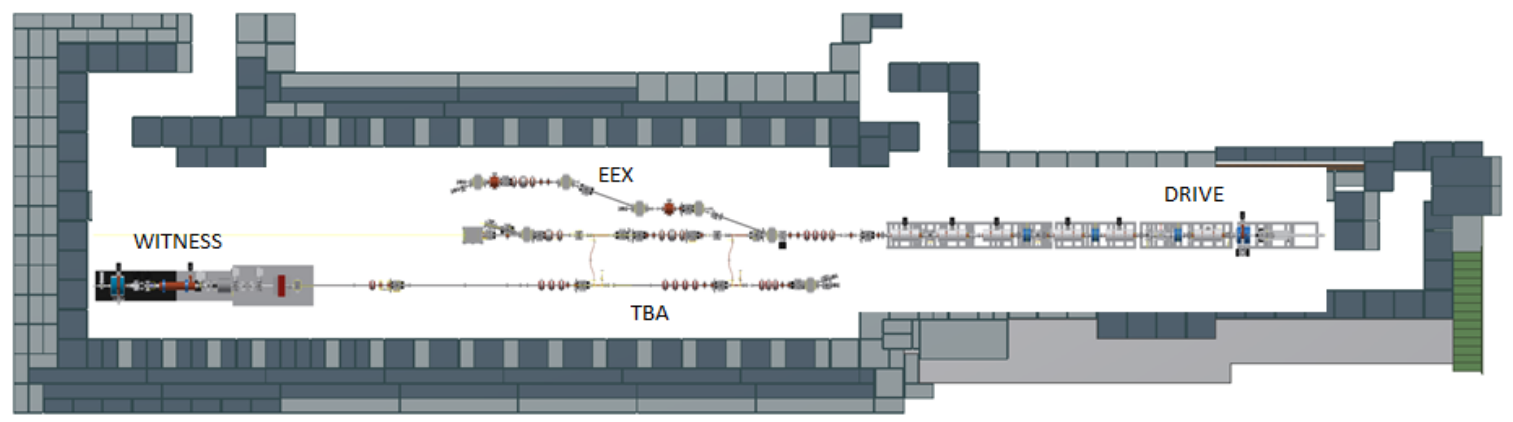
\includegraphics[width=\linewidth]{./images/bunker}
		\label{fig:bunker}
	\end{center}
\caption{AWA Facility bunker and layout. 
	The drive beam line (right) supplies high charge bunch trains at \SI{70}{MeV}.
	The witness beam line (left) supplies low charge one bunch at \SI{15}{MeV} }
\end{figure}
\begin{figure}[h]
	\begin{center}
		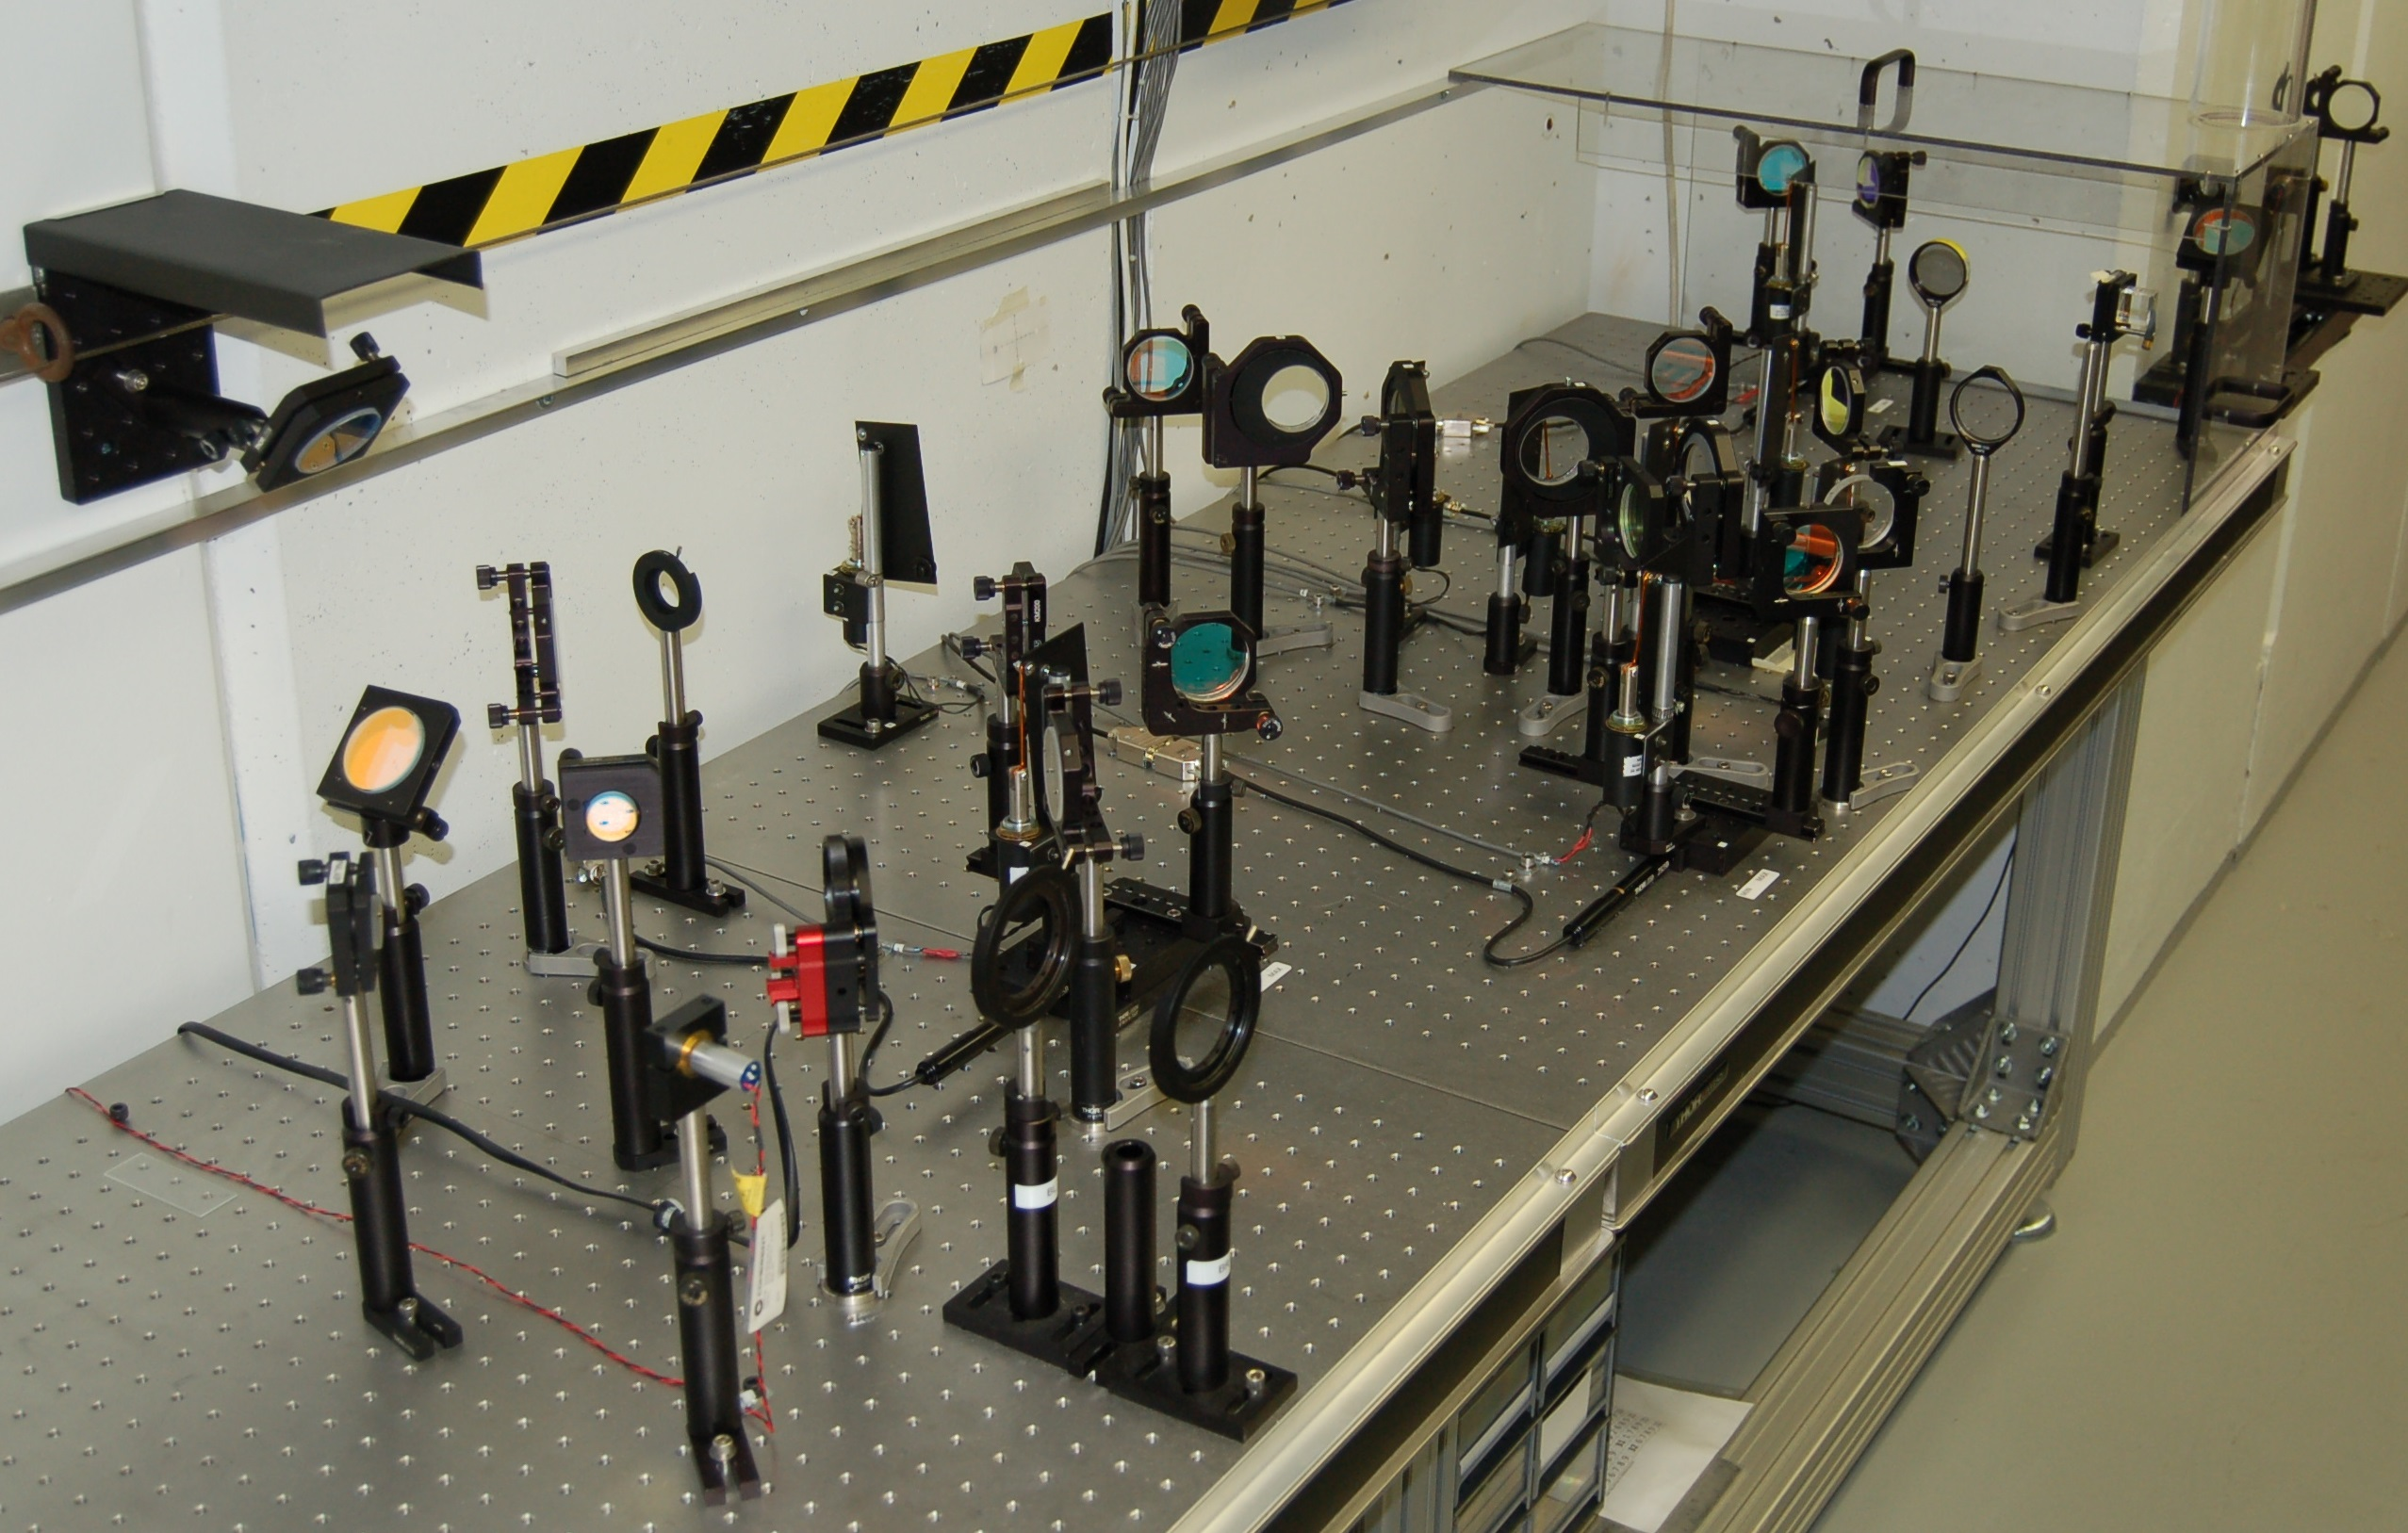
\includegraphics[width=0.5\textwidth]{images/multisplitter}\caption{UV multisplitter optics table.}
	\end{center}
	\label{fig:optics}
\end{figure}
\fi

The witness line rf photoinjector, located on the left side of Figure
1, uses a Mg cathode and the following linac consists of one copper
accelerating cavity. Prior to the multisplitter table, shown in
Fig. \ref{fig:optics}, the laser pulse is split between the drive and witness side.
This set up allows only one bunch per pulse on the witness line. Also
note that the beam from the drive line travels in the opposite direction
than the beam in the witness line. 

%%%%%%%%%%%%%%%%%%%%%%%%%%%%%%%%%%%%%%%%%%%%%%%%%%%%%%%%%%%%%%%%%%%%%%%%%%%%%%%%%%%%%%%%%%%%
%%%%%%%%%%%%%%%%%%%%%%%%%%%%%%%%%%%%%%%%%%%%%%%%%%%%%%%%%%%%%%%%%%%%%%%%%%%%%%%%%%%%%%%%%%%%
\Section{Dielectric Structures}

%%%%%%%%%%%%%%%%%%%%%%%%%%%%%%%%%%%%%%%%%%%%%%%%%%%%%%%%%%%%%%%%%%%%%%%%%%%%%%%%%%%%%%%%%%%%
%%%%%%%%%%%%%%%%%%%%%%%%%%%%%%%%%%%%%%%%%%%%%%%%%%%%%%%%%%%%%%%%%%%%%%%%%%%%%%%%%%%%%%%%%%%%
\Subsection{Power Generation}

\lsnote{Somewhere you need a comprehensive description of simplified staging vesus full staging.  I am not sure it is here, but it should be before you mention simplified staging.}

Currently, all \lsnote{define PETS acronym} PETS and accelerating structures installed in the AWA's
simplified staging scheme are metallic. It has been shown that a few
key equations can demonstrate the relationship between beam parameters
and the resulting \lsnote{\sout{rf} power} generated in the decelerating cavity. This section
borrows heavily from previous work at CLIC and the AWA \cite{key-3,key-8}. 
Starting with the timing, each bunch in the drive train will generate
an rf pulse of finite length in the structure. Each bunch is separated
in time by $T_{b}$, and the \lsnote{average?} beam current can be written as $I=\frac{Q}{T_{b}}$.
\lsnote{define Q, is it the charge per bunch?} The bunches are Gaussian in the longitudinal direction, and the form
factor, $\Phi$, is used to describe\lsnote{\sout{s}} the Gaussian shape by taking
the Fourier transform of the charge distribution: 
\begin{equation}
\Phi=exp\left[\frac{-(k_{z}\sigma_{z})^{2}}{2}\right]
\end{equation}
Where $k_{z}=\frac{2\pi}{\lambda_{z}}$ is the longitudinal wave number
and $\sigma_{z}$ is the rms bunch length. \lsnote{That was confusing.  You said phi was the FT of the charge distribution, but in the equation after that it looks like the charge distribution not the FT}  Note the subscript z \lsnote{indicates \sout{refers to the characteristics of the cavity and bunch in}} the longitudinal
direction. Then using the partial differential equation that relates
the power generated by the wakefield to the change in power over time, \lsnote{I would include the equation}
the power generated by a bunch train can be written as:
\begin{equation} \label{eq:rfpower}
P_{t}(t)=\frac{\omega_{z}\,L^{2}I^{2}}{4\,v_{g}}\frac{R}{Q_{d}}\left(\frac{1-e^{-\alpha L}}{\alpha L}\right)\Phi^{2}
\end{equation}
With $I$ being the beam current as defined above, $\alpha=\frac{\omega}{2Q_{d}v_{g}}$
being the attenuation constant \cite{key-9}, R is the shunt impedance
per unit length, and $Q_{d}$ is the quality factor for the decelerating
structure. \lsnote{You didn't define L or vg} Note, the derivation of equation 4 can be found in reference
\cite{key-8}, and due to the complex geometry of metallic structures,
the value of R/Q is often calculated in electromagnetic codes such
as CST Microwave Studio. 

\lsnote{You probably were intending to do this, but this section should close out with a predicted power generation 
in the decelerating structures.  The discussion of how that depends on number of bunches in the bunch train should be here as well.}

\Subsection{Accelerating Structures}

\Section{Two Beam Acceleration}

\Section{AWA Design Requirements} \label{sec:requirements}

\lsnote{This is probably where you should have the overview of simple staging versus full staging, and a summary of what was required to go to full staging.  The title of the section should also be changed, maybe `Fully staged two beam acceleration'?}

In order to design and test the desired beam line, three technologies 
new to the AWA were investigated. These include a kicker, septum magnets, 
and non-GA optimization algorithms.

% An example for enumerate
\begin{enumerate}
	\item Kicker Design
	\item Septum Design
	\item Optimization 
\end{enumerate}

% A quotation example
% Every quota must be accompanied by a reference to the source
% in a footnote or in the Bibliography
\begin{quotation}
	test
\end{quotation}


\Section{Thesis Outline}
